\chapter{AES}

\section{实验目的}

理解 AES 算法的不同工作模式。

\section{实验要求}
实现两个基于 AES 的加密/解密系统,一个在 CBC 模式下使用 AES,另
一个在 CTR 模式下使用 AES。 在这两种情况下,16 字节的初始向量 IV 都
是随机选择的,并已放在密文中。对于 CBC 加密,请使用课程中讨论的 PKCS5
填充方案。
以下提供了解密过程正确性的测试用例。测试用例包含了 AES 密钥和一个
密文(两者都是十六进制编码的),需要恢复出明文并在实验报告中展示结果。

\section{实验内容}


\subsection{程序设计与实现}

具体代码见附录\ref{appendix:aes},此处仅对关键设计进行说明。

由于需要对分组进行异或或者数加操作,笔者定义了函数byte\_xor和byte\_add。

由于需要使用PKCS5填充方案,笔者定义了函数msg\_block\_generator和cipher\_block\_generator
用于填充。

笔者给出两个类CBC和CRT分别代表两种分组模式,包含方法encrypt和decrypt。
如图\ref{fig:aes}所示,以ECB, CRT和CBC的加密模式为例,可以看到ECB模式中的分组加密可以应用到
CTR模式和CBC模式中。按照实验要求,在CRT模式和CBC模式的加密过程中,
可直接调用Crypto库中的AES类使用其ECB模式块进行代码简化。解密同理。

\begin{figure}[!htbp]
    \centering
    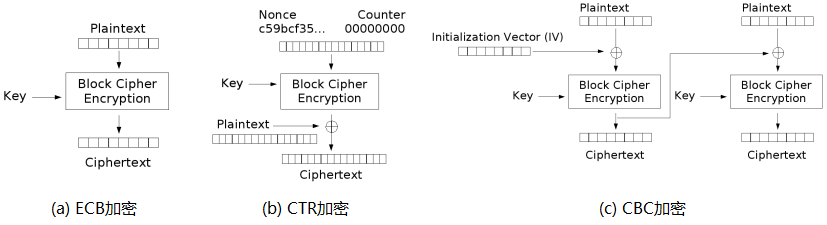
\includegraphics[width=1\textwidth]{figures/aes.png}
    \caption{ECB, CRT, CBC加密模式对比}
    \label{fig:aes}
\end{figure}

\subsection{恢复明文结果}

四组数据的解密结果分别为:

Basic CBC mode encryption needs padding.

Our implementation uses rand. IV

CTR mode lets you build a stream cipher from a block cipher.

Always avoid the two time pad!